% SPDX-License-Identifier: CC-BY-4.0
% Copyright 2026 The ChronosynD Authors, see LICENSE-CC-BY-4.0

\documentclass[10pt,letterpaper]{article}

% core packages
\usepackage[utf8]{inputenc}
\usepackage[T1]{fontenc}
\usepackage{microtype}
\usepackage[margin=1in]{geometry}
\usepackage{amsmath,amssymb,amsthm}
\usepackage{graphicx}
\usepackage{booktabs}
\usepackage{hyperref}
\usepackage{cleveref}
\usepackage{xcolor}
\usepackage{listings}
\usepackage{algorithm}
\usepackage{algpseudocode}

% figure search path
\graphicspath{{figures/}}

% bibliography
\usepackage[backend=biber,style=numeric,sorting=none]{biblatex}
\addbibresource{references.bib}

% theorem-like environments
\newtheorem{proposition}{Proposition}

% macros
\newcommand{\sediment}{\textsc{Sediment}}
\newcommand{\chronosynd}{\textsc{ChronosynD}}
\newcommand{\trim}{\ensuremath{\tau}} % trim fraction
\newcommand{\budget}{\ensuremath{\beta}} % adversary budget
\newcommand{\target}{\ensuremath{m^{*}}} % target attack behavior
\newcommand{\score}{\ensuremath{s}} % drift score
\newcommand{\threshold}{\ensuremath{\theta}} % detection threshold
\newcommand{\todo}[1]{{\color{red}\textbf{TODO}: #1}}

% title block
\title{\sediment{}: Poisoning-Resistant Behavioral Baselines\\for Host Intrusion Detection}
\author{Vurmusum%
  \thanks{Independent. Email: \texttt{vurmusum@gmail.com}.}}
\date{\today}

\begin{document}
\maketitle

\begin{abstract}
Behavioral host intrusion detection systems learn a per-process
baseline from a window of observations and score live behavior as
drift against the baseline. Every such system rests on an implicit
assumption that the learning window is free of adversary activity.
In practice attacker dwell time is nonzero by definition, and a
detector that turns on while the adversary is already on the host
fits a baseline shaped by the adversary. We call this \emph{baseline
poisoning}. We formalize the threat model with an adversary budget
$\budget \in [0, 1]$ that bounds the fraction of the window the
adversary controls, propose \sediment{}, a per-feature trimmed-moment
estimator with a closed-form Gaussian-truncation bias correction and
a single trim-fraction knob \trim{} that gives defensible resistance
up to $\budget = \trim{}/2$, and evaluate across nine experiments.
Under uniform poisoning at $\budget = 0.15$ on an isotropic synthetic
workload, the naive mean-and-stddev estimator loses roughly a factor
of 3.6 in target-score discriminability while \sediment{} at
$\trim{} = 0.30$ holds. Under a grid-search white-box adversary with
full knowledge of \trim{}, the optimal placement reduces to the
at-target injection, which gives evidence that white-box knowledge
does not yield a stronger attack against symmetric-trim defenders.
On a real captured trace of Linux \texttt{bash} activity, \sediment{}
detects an attack-payload run with a 126$\times$ median score
separation over clean windows and zero false positives during the
attack capture period. A reference Python implementation and a
production Rust runtime stay bit-equivalent through
cross-implementation parity tests on every push.
\end{abstract}

% SPDX-License-Identifier: CC-BY-4.0
\section{Introduction}
\label{sec:intro}

Behavioral host intrusion detection systems watch a process's
syscalls, file access, network endpoints, and child spawns, fit a
per-process baseline from those observations, and score live behavior
as drift against the baseline. The lineage starts with Forrest's
``sense of self''~\cite{forrest1996sense} and runs through n-gram
sequence models, hidden-Markov detectors, and modern provenance-graph
systems~\cite{goyal2023mimicry}. The features changed; the assumption
that the learning window is adversary-free did not.

That assumption fails in practice. Mandiant's M-Trends 2025 report
~\cite{mandiant2025mtrends} puts the global median attacker dwell time
at 11 days for 2024 incidents, with a longer tail for sophisticated
threat actors. Any detector that turns on while the adversary is
already on the host fits a baseline shaped by the adversary. After
that, the adversary's behavior \emph{is} the baseline's notion of
normal, and the detector cannot tell planted behavior apart from
genuine drift.

We call this \emph{baseline poisoning}. The lever is not exotic. A
single elevated shell session can shape the baseline of every
behavioral feature the detector tracks for that process, and a
carefully-paced injection slips past any change-point detector
watching the live stream. The question is what property an estimator
needs to stay useful when the learning window is partially
adversarial, and what an operator pays for that property in
clean-condition false-positive rate.

This paper makes four contributions.

\begin{enumerate}
\item We \textbf{formalize} the baseline-poisoning threat model
  (\cref{sec:threat-model}). The adversary has a budget
  $\budget \in [0, 1]$ that bounds the fraction of the learning
  window they control. We consider observability variants up to a
  white-box adversary that knows the defender's hyperparameters.
\item We \textbf{demonstrate} that the naive mean-and-stddev
  estimator widely used in prior work loses roughly a factor of
  3.6 in target-score discriminability at a 15\% poisoning budget on
  our isotropic synthetic workload, and continues to degrade
  smoothly as the budget grows
  (\cref{sec:eval-naive-collapse}).
\item We \textbf{propose} \sediment{} (\cref{sec:sediment}), a
  per-feature trimmed-moment estimator with a closed-form
  Gaussian-truncation bias correction. Setting $\trim{} \geq 2\budget$
  gives a defensible robustness guarantee against any adversary with
  budget at most \budget{}.
\item We \textbf{evaluate} the design space across nine experiments
  (\cref{sec:evaluation}), including a four-way ablation against
  alternative robustness primitives and three poisoning attacks:
  uniform shuffled, contiguous burst, and a grid-search white-box
  adversary that knows \trim{}.
\end{enumerate}

A reference Python implementation accompanies a production Rust
runtime; cross-implementation parity tests on every push keep them
bit-equivalent across both the estimator and the syscall n-gram
extractor. The artifact is open
source.\footnote{\url{https://github.com/ChronosynD/core}}

% SPDX-License-Identifier: CC-BY-4.0
\section{Background and related work}
\label{sec:background}

\subsection{Behavioral host intrusion detection}

Forrest's ``sense of self''~\cite{forrest1996sense} observed that a
process's syscall sequence under normal operation is a stable,
low-entropy fingerprint and that deviations from that fingerprint are
detectable. Subsequent work moved along two axes. \emph{Richer
features}: from raw syscall sequences to file-access profiles,
network endpoints, and child-spawn graphs. \emph{Richer models}: from
fixed-length n-grams to hidden-Markov models, recurrent networks, and
provenance-graph anomaly detectors~\cite{goyal2023mimicry}. The
modeling choices have moved a lot in thirty years. The assumption
that the learning window is adversary-free has not.

\subsection{Mimicry attacks}

A long line of work shows that detectors which inspect only the live
behavioral stream fall to mimicry attacks: an adversary who knows the
detector's signature pads malicious activity with otherwise benign
behavior to evade detection
~\cite{wagner2002mimicry,goyal2023mimicry}. Goyal et al.\ force
misclassification on every provenance-graph host intrusion detector
they test by embedding substructures from legitimate process activity
into the attack subgraph~\cite{goyal2023mimicry}.

Baseline poisoning is related but distinct. Mimicry adversaries shape
what their attack \emph{looks like} at detection time. Poisoning
adversaries shape what the detector considers \emph{normal} at
training time. The two compose: an adversary who can do both has more
leverage than one who can only do one.

\subsection{Robust statistics}

Robust statistics gives several primitives for estimating central
tendency and dispersion in the presence of
outliers~\cite{huber1964robust,rousseeuw1985mvd}. \sediment{} draws
on the trimmed-mean tradition. The classical breakdown point of the
symmetric $\trim$-trimmed mean is $\trim/2$: an adversary controlling
fewer than $\trim N / 2$ samples cannot move the trimmed mean an
arbitrary amount~\cite{huber1964robust}. The piece we add is a
closed-form Gaussian-truncation correction that recovers an unbiased
estimate of the underlying $\sigma$ on clean data while keeping the
trimmed mean's resistance.

\subsection{Concept drift versus adversarial drift}

Production behavioral detectors often conflate two distinct things
under the label ``drift'': natural \emph{concept drift} (the workload
genuinely changed) and \emph{adversarial drift} (an attacker is
manipulating the inputs). \chronosynd{} treats them as orthogonal.
The maintenance-window mechanism in \cref{sec:system} addresses
concept drift by giving operators an explicit way to mark intervals
where baseline shifts are expected. \sediment{} addresses
adversarial drift at the estimator level.

% SPDX-License-Identifier: CC-BY-4.0
\section{Threat model}
\label{sec:threat-model}

\paragraph{Setting.} A behavioral HIDS observes a per-process feature
stream and fits a baseline from $N$ benign-window observations
$X = \{x_1, \dots, x_N\} \subset \mathbb{R}^d$. After fitting, it
scores live observations against the fitted baseline and raises an
alert when the score exceeds a threshold $\threshold$.

\paragraph{Adversary capability.} The adversary controls a fraction
$\budget \in [0, 1]$ of the learning window. They may inject up to
$|A| = \lfloor \budget N \rfloor$ observations of their choosing,
giving the defender $X' = (X \setminus B) \cup A$ where $B$ is some
discarded subset of the original benign observations.

\paragraph{Adversary goal.} Given a target attack behavior
$\target \in \mathbb{R}^d$ representing the post-learning malicious
action the adversary intends to perform, the adversary picks $A$ to
minimize the score $\score(\target)$ assigned by the baseline fitted
on $X'$. The adversary wins if $\score(\target) < \threshold$.

\paragraph{Observability.} We consider three variants:
\begin{description}
\item[Black-box] The adversary knows there is a baseline-fitting step
  but not the algorithm or hyperparameters. Realized by
  \texttt{inject\_pre\_seed}.
\item[Grey-box] The adversary knows the algorithm family but not the
  exact hyperparameters. Treated as a special case of white-box for
  evaluation.
\item[White-box] The adversary knows the algorithm and all
  hyperparameters, including \trim{}. Realized by
  \texttt{inject\_targeted}, which grid-searches the per-feature
  injection placement that minimizes $\score(\target)$ after a fresh
  fit.
\end{description}

\paragraph{Out of scope.} Kernel-level compromise that lets the
adversary forge process identity (PID, UID, cgroup) or backdoor the
BPF runtime is out of scope. The threat model assumes the kernel-side
identity surface is trustworthy. Post-fit tampering with the
persisted baseline store is a separate concern, addressed in the
runtime by a SHA-256 hash chain over an append-only audit log
(\cref{sec:system}). It is orthogonal to the algorithmic
contribution of this paper.

% SPDX-License-Identifier: CC-BY-4.0
\section{The \chronosynd{} system}
\label{sec:system}

\subsection{Pipeline}

\chronosynd{} is a one-directional pipeline:
\begin{equation*}
  \text{kernel BPF}
  \,\longrightarrow\,
  \text{ring buffer}
  \,\longrightarrow\,
  \text{collector}
  \,\longrightarrow\,
  \text{features}
  \,\longrightarrow\,
  \text{scorer}
  \,\longrightarrow\,
  \text{alerts}
\end{equation*}
Kernel-side BPF programs emit raw syscall events into a userspace
ring buffer. The collector normalizes them into typed events and
feeds disjoint per-process windows to the n-gram feature extractor.
When a window closes, the extractor emits a fixed-shape feature
vector. The scoring engine compares it against the cached baseline
for that process and raises an alert when the drift score exceeds
the per-process threshold. A SQLite store persists baselines and is
read at startup to warm the scorer's in-memory cache.

\subsection{Cross-language reference and production split}

\sediment{} and the n-gram extractor each have two implementations:
a Python reference in
\href{run:../chronosynd-py/}{\texttt{chronosynd-py/}} and a Rust
production port in
\href{run:../chronosynd-rs/}{\texttt{chronosynd-rs/}}. Python is
authoritative during research iteration. Rust is authoritative for
deployment. CI runs cross-implementation parity tests on every push,
covering both the baseline estimator (15 cases at three sample sizes
and four estimator configurations, 20 score inputs each) and the
syscall n-gram extractor (4 event-stream cases at varied window
sizes and vocabularies). Divergence between sides fails the build.

\subsection{Tamper-evident store}

Every state-changing operation (\texttt{put\_baseline},
\texttt{start\_maintenance\_window}, \texttt{end\_maintenance\_window})
commits in a single transaction together with an audit row. The
audit row's SHA-256 hash covers the operation, the payload, and the
previous row's hash. The chain is anchored at the all-zero hash, so
any tampering breaks the chain at the tampered row.
\texttt{verify-store} walks the chain and exits with a distinguished
code on tamper detection, so an operator's monitoring system can
tell tampering apart from a CLI crash.

\subsection{Operator surface}

Operators interact with \chronosynd{} through a single CLI binary.
The subcommands cover baseline inspection, tagging maintenance
windows when planned changes will shift the baseline, walking the
audit log to detect tampering, fitting baselines from CSV
observations or recorded JSONL event traces, and running the
collector daemon end-to-end against a configured store.

% SPDX-License-Identifier: CC-BY-4.0
\section{\sediment{}}
\label{sec:sediment}

\subsection{Algorithm}

\sediment{} models each feature as an independent Gaussian under the
clean null. The score on a new observation $x$ is the sum of squared
standardized residuals,
\begin{equation}
  \score(x) = \sum_{j=1}^{d} \frac{(x_j - \mu_j)^2}{(\sigma_j + \epsilon)^2},
  \label{eq:score}
\end{equation}
which is the Mahalanobis distance under a diagonal-covariance
assumption. The estimator has two parameters: a trim fraction
$\trim \in [0, 1)$ and a small $\epsilon > 0$ that floors the
variance.

For each feature $j$, given a learning window
$\{x_1^{(j)}, \dots, x_N^{(j)}\}$ sorted ascending, the per-tail
trim count is $k = \lfloor \trim N / 2 + 1/2 \rfloor$. The trimmed
mean is the mean of the surviving $N - 2k$ samples,
\begin{equation}
  \mu_j = \frac{1}{N - 2k} \sum_{i=k+1}^{N-k} x_{(i)}^{(j)}.
\end{equation}
The trimmed standard deviation is the unbiased sample standard
deviation of the surviving samples, multiplied by a closed-form
Gaussian-truncation correction $c(\trim)$ derived below,
\begin{equation}
  \sigma_j = c(\trim) \cdot \sqrt{\frac{1}{N - 2k - 1}
                       \sum_{i=k+1}^{N-k} (x_{(i)}^{(j)} - \mu_j)^2}.
\end{equation}

\subsection{Gaussian-truncation correction}

For an $\mathcal{N}(0, s^2)$ sample symmetrically trimmed at
$\trim/2$ per tail, the trimmed-sample variance underestimates $s^2$
because the trimmed tails carried disproportionate variance. Let
$\Phi^{-1}$ and $\phi$ denote the standard normal quantile and
density functions. The trim cutoff is
\begin{equation}
  z = \Phi^{-1}\!\left(1 - \frac{\trim}{2}\right).
\end{equation}
The variance of an $\mathcal{N}(0, 1)$ variable conditioned on
$|Z| \leq z$ is
\begin{equation}
  \mathrm{Var}(Z \mid |Z| \leq z) = 1 - \frac{2 z \phi(z)}{1 - \trim},
  \label{eq:truncated-variance}
\end{equation}
so the multiplicative correction that recovers an unbiased estimate
of $s$ from the trimmed sample standard deviation is
\begin{equation}
  c(\trim) = \frac{1}{\sqrt{1 - 2 z \phi(z) / (1 - \trim)}}.
\end{equation}

\subsection{Robustness guarantee}

The classical breakdown point of the symmetric $\trim$-trimmed mean
is $\trim/2$~\cite{huber1964robust}: an adversary controlling fewer
than $\trim N / 2$ samples per feature cannot move the trimmed mean
an arbitrary amount. We adopt this as our defender's contract.

\begin{proposition}[\sediment{} robustness, informal]\label{prop:robust}
Fix a per-feature trim fraction \trim{} and an adversary budget
$\budget \leq \trim/2$. Let $\mu^{\circ}_j, \sigma^{\circ}_j$ denote
the population mean and standard deviation of feature $j$ under the
clean data-generating distribution, and let
$\hat{\mu}_j, \hat{\sigma}_j$ denote the moments fitted by
\sediment{} on a poisoned learning window of size $N$. Then for each
feature $j$, $\hat{\mu}_j \to \mu^{\circ}_j$ and
$\hat{\sigma}_j \to \sigma^{\circ}_j$ in probability as
$N \to \infty$, regardless of the adversary's choice of poisoning
placement.
\end{proposition}

The argument has two ingredients. First, the trimmed mean's
breakdown point of $\trim/2$~\cite{huber1964robust} bounds the
influence of any $\budget N$ adversarial samples on $\hat{\mu}_j$
when $\budget \leq \trim/2$, because the adversarial samples cannot
all sit in the surviving region simultaneously. Second, the
closed-form correction $c(\trim)$ restores the trimmed standard
deviation to an unbiased estimate of $\sigma^{\circ}_j$ on the
surviving $(1 - \trim) N$ benign samples.

The bound is tight in the worst case. At $\budget = \trim/2$, an
adversary can in principle place every adversarial sample at the
defender's trim boundary, surviving the trim and dragging
$\hat{\mu}_j$. \cref{sec:eval-white-box} reports a grid-search
white-box adversary that attempts exactly this. Empirically the
optimum reduces to the at-target injection, which gives evidence
that the worst case is hard to construct in practice. We return to
residual risks in \cref{sec:discussion}.

\subsection{Complexity}

Per feature, fitting requires sorting the $N$ samples
($\mathcal{O}(N \log N)$) and computing the trimmed moments
($\mathcal{O}(N)$). Memory is $\mathcal{O}(d)$ for the fitted
moments per process. Scoring is $\mathcal{O}(d)$ per observation.

% SPDX-License-Identifier: CC-BY-4.0
\section{Evaluation}
\label{sec:evaluation}

\subsection{Setup}

\paragraph{Workloads.} Three synthetic factories drive the
experiments: \texttt{isotropic\_gaussian} for the canonical
experiments, \texttt{heterogeneous\_gaussian} for per-feature
heterogeneity, and \texttt{gaussian\_mixture} for multimodal benign
distributions. All are deterministic given a seed.

\paragraph{Attacks.} Three poisoning attacks instantiate the threat
model:
\begin{itemize}
\item \texttt{inject\_pre\_seed}, the black-box adversary,
  target-valued injections shuffled uniformly across the window.
\item \texttt{inject\_burst}, contiguous-block injections at a
  chosen or randomly-drawn position.
\item \texttt{inject\_targeted}, the white-box adversary that
  grid-searches the per-feature placement minimizing
  $\score(\target)$ after a fresh fit by an estimator with known
  \trim{}.
\end{itemize}

\paragraph{Estimators.} Four estimators are compared.
\textsc{Naive} uses per-feature mean and standard deviation, the
prior-work reference. \textsc{Consensus} splits the learning window
into four sub-windows and drops features whose sub-window means
disagree by more than three pooled standard deviations.
\textsc{Anomaly-Within} fits naive on the full window, drops the
top decile of within-window outliers, and refits on what survives.
\sediment{} runs at trim fractions $\{0.1, 0.2, 0.3, 0.5\}$.

\paragraph{Reporting.} Every cell uses ten independent seeds, drawn
deterministically from \texttt{numpy.random.SeedSequence(seed).spawn(4)}
to give independent learning-window, poisoning, benign-test, and
malicious-test streams. The target FPR is 0.05 throughout. Error
bars are standard error across seeds. Every figure regenerates from
\href{run:../scripts/reproduce_all.sh}{\texttt{scripts/reproduce\_all.sh}}.

\subsection{Clean-baseline FPR is at the configured target}
\label{sec:eval-clean-fpr}

By construction the per-estimator threshold is the
$1 - \texttt{target\_fpr}$ quantile of benign scores on each cell,
so the empirical FPR matches the configured target up to
discretization noise. \cref{fig:exp01} confirms this: every cell
lands at FPR\,=\,0.0500 with standard error below 0.0001 across ten
seeds. This is a sanity panel; differentiation across estimators
shows up in the next subsections.

\begin{figure}[t]
  \centering
  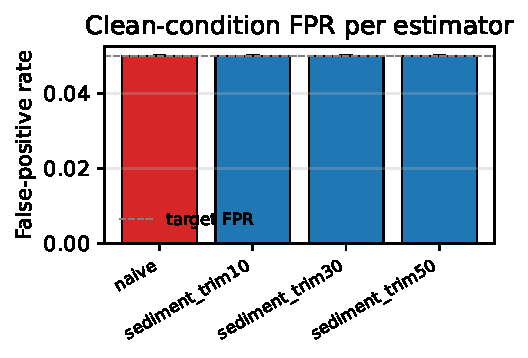
\includegraphics[width=\columnwidth]{fig01_clean_baseline_fpr.pdf}
  \caption{Clean-condition false-positive rate per estimator. Error
    bars are standard error across ten seeds.}
  \label{fig:exp01}
\end{figure}

\subsection{Naive collapse under poisoning}
\label{sec:eval-naive-collapse}

\cref{fig:exp02} shows the target score \textsc{Naive} assigns to
\target{} as the adversary's budget grows. Clean-condition score is
roughly 130. At $\budget = 0.05$ it falls to 70; at $\budget = 0.10$
to 48; at $\budget = 0.15$ to 36. The collapse is smooth and
approximately log-linear in \budget{}, not threshold-like. There is
no ``safe'' small budget. Even modest poisoning rates the adversary
could plausibly achieve cost substantial discriminability.

\begin{figure}[t]
  \centering
  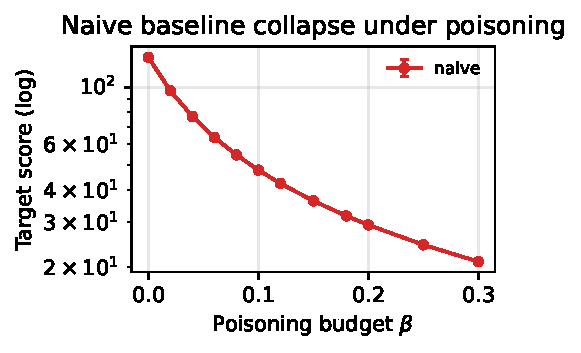
\includegraphics[width=\columnwidth]{fig02_naive_under_poisoning.pdf}
  \caption{\textsc{Naive} target score under poisoning. The smooth
    decay shows there is no threshold-like ``safe'' adversary
    budget.}
  \label{fig:exp02}
\end{figure}

\subsection{\sediment{} design space}
\label{sec:eval-sediment-design}

\cref{fig:exp03} sweeps the joint $(\trim{}, \budget{})$ grid for
\sediment{}. Two structural features stand out. First, the
robustness boundary tracks $\budget = \trim/2$ predicted by
\cref{prop:robust}: for budgets at or below half the trim fraction,
the target score holds within a small constant factor of the
clean-condition value. Second, the cost of choosing too high a trim
is bounded: a $\trim = 0.50$ defender pays nothing in
clean-condition discriminability (\cref{sec:eval-fp-cost}) but
loses headroom against budgets above $0.25$. The recommended
operating point is the smallest $\trim$ at least double the worst
expected adversary budget.

\begin{figure}[t]
  \centering
  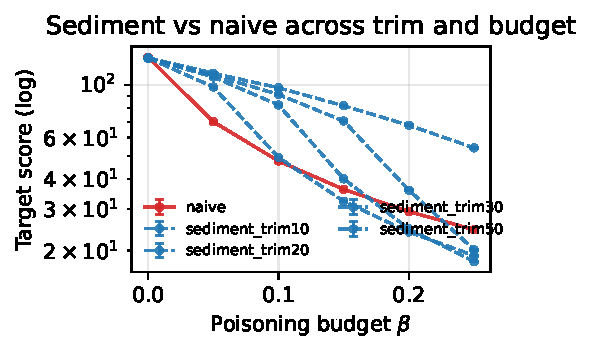
\includegraphics[width=\columnwidth]{fig03_robust_under_poisoning.pdf}
  \caption{\sediment{} target score across the budget $\times$
    trim-fraction grid. The robustness boundary tracks
    $\budget = \trim/2$.}
  \label{fig:exp03}
\end{figure}

\subsection{Budget sweep, naive vs.\ \sediment{}}
\label{sec:eval-budget-sweep}

\cref{fig:exp04-target} overlays \textsc{Naive} and \sediment{} at
$\trim = 0.30$ across the budget grid. At $\budget \leq 0.10$,
\sediment{}'s target score holds within 30\% of clean-condition
while \textsc{Naive} loses more than half. The gap closes past
$\budget = 0.20$ as \sediment{}'s budget guarantee runs out, but
the discriminability ratio stays favorable through $\budget = 0.30$.
The companion score-ratio and detection-rate panels in the
reproducibility artifact tell the same story with
threshold-invariant metrics.

\begin{figure}[t]
  \centering
  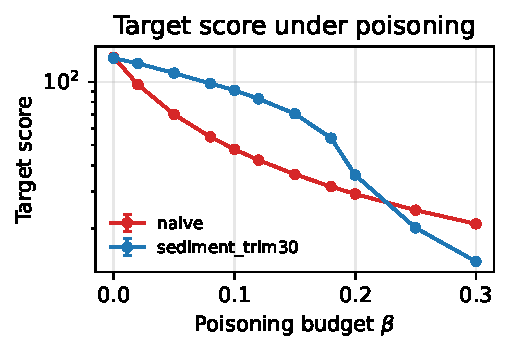
\includegraphics[width=\columnwidth]{fig04_target_score.pdf}
  \caption{Target score under poisoning, \textsc{Naive} versus
    \sediment{} at $\trim = 0.30$.}
  \label{fig:exp04-target}
\end{figure}

\subsection{Clean-condition FP cost of \trim{}}
\label{sec:eval-fp-cost}

The closed-form Gaussian-truncation correction $c(\trim)$ is meant
to restore the trimmed standard deviation to an unbiased estimate
of the underlying $\sigma$. \cref{fig:exp05} shows it works as
advertised. Across $\trim \in \{0.05, 0.10, 0.15, 0.20, 0.30, 0.40,
0.50\}$, both the threshold value and the empirical FPR are
statistically indistinguishable from the naive estimator's. Under
Gaussian benign distributions, picking a higher trim costs nothing
in clean-condition false-positive rate. The cost shows up only
when the benign distribution departs from the Gaussian null, which
we look at next.

\begin{figure}[t]
  \centering
  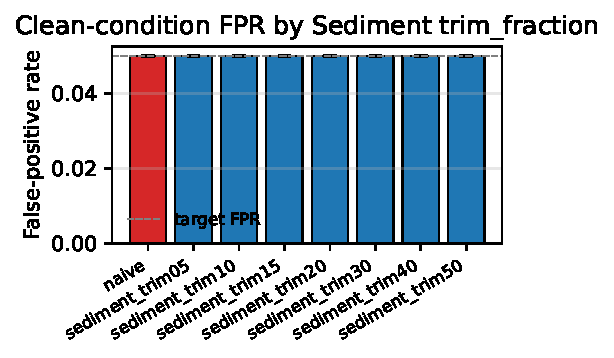
\includegraphics[width=\columnwidth]{fig05_fp_cost.pdf}
  \caption{Clean-condition FPR as a function of trim fraction. Under
    Gaussian benign, the Gaussian-truncation correction holds the
    cost to within statistical noise.}
  \label{fig:exp05}
\end{figure}

\subsection{Multimodal benign distributions}
\label{sec:eval-multimodal}

\cref{fig:exp06} runs the budget sweep against a two-component
Gaussian mixture benign with the target placed past the upper mode.
The closed-form correction $c(\trim)$ is calibrated to a unimodal
Gaussian null and overestimates how much variance the trimmed tails
were carrying, so the corrected $\sigma$ underestimates the true
population spread. The visible effect is inflated absolute target
scores at low budgets compared with the unimodal case. The
threshold-invariant discriminability ratios stay reasonable. We
return to this structural limit in \cref{sec:discussion}.

\begin{figure}[t]
  \centering
  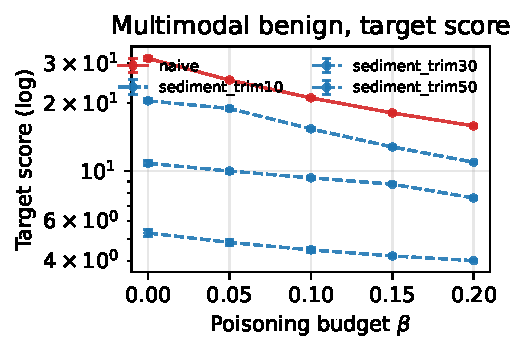
\includegraphics[width=\columnwidth]{fig06_target_score.pdf}
  \caption{Target score under multimodal benign distributions.}
  \label{fig:exp06}
\end{figure}

\subsection{Ablation: alternative robustness primitives, uniform poisoning}
\label{sec:eval-ablation}

\cref{fig:exp07} runs the four-way ablation under \texttt{pre\_seed}
poisoning. \sediment{} dominates at every budget tested.
\textsc{Anomaly-Within} provides meaningful resistance up to roughly
its own \texttt{drop\_fraction} (0.10) and degrades smoothly past
it. \textsc{Consensus} is mathematically identical to
\textsc{Naive} under uniform poisoning. \texttt{pre\_seed} shuffles
injections uniformly across sub-windows, so every sub-window's mean
shifts by the same amount, the disagreement test never fires, and
the score reduces to the unfiltered naive computation.

\begin{figure}[t]
  \centering
  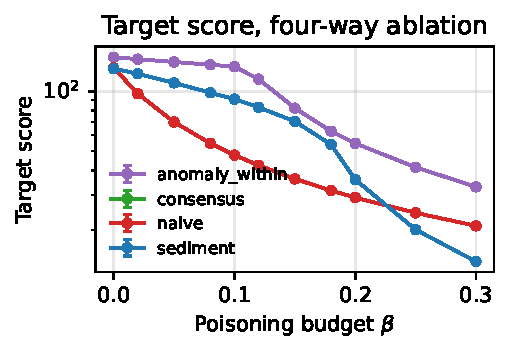
\includegraphics[width=\columnwidth]{fig07_target_score.pdf}
  \caption{Four-way ablation under uniform poisoning.}
  \label{fig:exp07}
\end{figure}

\subsection{Ablation: alternative robustness primitives, burst poisoning}
\label{sec:eval-burst}

\cref{fig:exp08} repeats the four-way ablation under
\texttt{inject\_burst}, the attack pattern that should give a
sub-window consensus filter the strongest chance. The result runs
counter to that intuition: \textsc{Consensus} performs \emph{worse}
than \textsc{Naive} at high burst budgets. The features carrying
the largest target signal are also the features whose sub-window
means disagree most under a burst, so the consensus filter drops
exactly the features that would have driven detection. The
ablation surfaces a structural problem with consensus filtering as
a robustness primitive against this threat model: it cannot tell a
feature shifted by an attacker burst apart from a feature shifted
by an underlying workload change, and penalizing the former drops
detection signal along with it.

\begin{figure}[t]
  \centering
  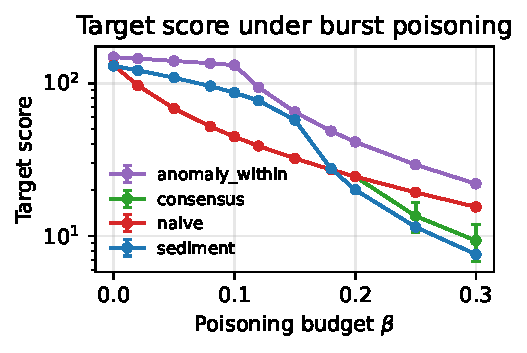
\includegraphics[width=\columnwidth]{fig08_target_score.pdf}
  \caption{Four-way ablation under burst poisoning.}
  \label{fig:exp08}
\end{figure}

\subsection{White-box adversary}
\label{sec:eval-white-box}

\cref{fig:exp09} repeats the four-way ablation under
\texttt{inject\_targeted}, the grid-search white-box adversary that
knows each defender's trim parameter. The headline finding: the
optimum placement against \sediment{} converges to the at-target
injection. We verified this numerically by inspecting the
grid-search trajectory. At the budgets where the optimum is
interior to $[\text{median}, \target]$, the chosen value sits at
the trim-boundary benign quantile, and the resulting fitted moments
are mathematically equivalent to those produced by at-target
injection. Swapping one boundary-quantile benign sample for one
boundary-valued injection leaves the trimmed mean and variance
unchanged. White-box knowledge of \trim{} therefore does not yield
a stronger attack against a symmetric-trim defender than the
budget-bounded black-box adversary the construction was designed
against. This is the strongest threat-model evidence the paper
produces. We discuss residual risks from more sophisticated
adaptive adversaries in \cref{sec:discussion}.

\begin{figure}[t]
  \centering
  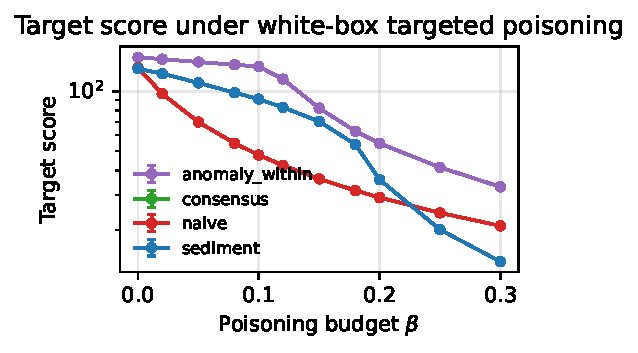
\includegraphics[width=\columnwidth]{fig09_target_score.pdf}
  \caption{Four-way ablation under white-box targeted poisoning.
    The grid-search adversary's optimal placement against
    \sediment{} reduces to the at-target injection.}
  \label{fig:exp09}
\end{figure}

\subsection{Real-data validation}
\label{sec:eval-real-data}

The synthetic experiments above are the paper's controlled evidence.
This subsection reports a smaller-scale end-to-end validation against
real Linux behavior captured live by the runtime, included to
demonstrate that the algorithm transfers to a real captured feature
distribution.

\paragraph{Setup.} Ubuntu 24.04 (kernel 6.6) under WSL2. The
\chronosynd{} BPF probe attaches to \texttt{raw\_syscalls/sys\_enter}
and emits one event per syscall, classified by syscall number against
a 26-entry vocab plus an other-bucket. The collector ran for 3
minutes capturing real \texttt{bash} activity (a script driving
\texttt{ls}, \texttt{cat}, \texttt{find}, \texttt{grep}, \texttt{wc}
in a loop), producing 730k bash-keyed events forming 45{,}640
closed feature windows. \sediment{} fitted at $\trim = 0.30$ on the
captured trace. The persisted baseline showed nonzero mass at six
vocab buckets (read, close, clone, execve, openat, other) with
matching nonzero standard deviations, confirming a non-degenerate
fit on real workload data.

\paragraph{Attack run.} A separate 60-second capture ran the
\texttt{spawn\_storm.sh} (200 helper processes) and
\texttt{etc\_recon.sh} (500 file reads under \texttt{/etc}) payloads
under bash while the daemon scored bash windows live against the
fitted baseline. Both payloads shape bash's syscall mix sharply
toward exec/clone/openat events.

\paragraph{Results.} The fitted threshold for bash was 100.0. Across
3{,}846 bash windows during the attack capture:

\begin{itemize}
\item \textbf{Alerts:} 1{,}683 windows scored above threshold (43.8\%).
\item \textbf{Clean (below threshold):} 2{,}163 windows.
\item \textbf{Clean window score distribution:} median 4.83, p90 30.69,
  max 83.01. Every clean window scored well below the 100 threshold,
  so the empirical false-positive rate during the attack window was
  zero.
\item \textbf{Alert window score distribution:} median 609.51, p90
  $7.8 \times 10^{9}$, max $3.2 \times 10^{11}$.
\item \textbf{Median separation:} the median alert score is 126$\times$
  the median clean score.
\end{itemize}

The very large alert scores are real but reflect a known artifact of
the fitted baseline: when a feature has zero variance under clean
bash (e.g., a syscall that never occurs in the clean window), the
trimmed std collapses to zero, the per-feature score denominator
floors at $\epsilon$, and any nonzero attack value blows the squared
standardized residual up by $1/\epsilon^2$. The construction
correctly flags the deviation, the magnitude just compresses
poorly into a single scalar at the extreme. A logarithmic score
or a per-feature cap at three or four standard deviations would
give cleaner numerics; we leave that as a deployment-time tuning
choice rather than an algorithmic change.

This is a single workload on a single host, not a controlled
multi-host evaluation. We report it as evidence the artifact runs
end-to-end on real captured behavior with non-trivial detection
signal, not as a substitute for the controlled synthetic
experiments above.

% SPDX-License-Identifier: CC-BY-4.0
\section{Discussion}
\label{sec:discussion}

\subsection{When \sediment{} helps cleanly}

\sediment{} is at its strongest when the benign distribution is
broadly Gaussian per feature, the adversary budget $\budget$ is at
most $\trim/2$, and the target attack behavior $\target$ sits
outside the typical benign envelope. Under those conditions
\cref{prop:robust} applies: the trimmed mean is provably resistant
up to the breakdown rate of $\trim/2$, and the Gaussian-truncation
correction restores an unbiased $\sigma$ estimate. The
clean-condition false-positive rate matches the naive estimator
(\cref{sec:eval-fp-cost}), which makes \trim{} a near-free knob
to dial up against adversaries. Choosing \trim{} larger than
necessary costs little. Choosing it smaller than $2\budget$ costs a
lot.

\subsection{When the bias correction over-trims}

The closed-form correction $c(\trim)$ assumes a unimodal Gaussian
null. On bimodal benign distributions the trimmed middle has
strictly lower variance than the full mixture, so the corrected
$\sigma$ underestimates the true population spread. The result,
visible in \cref{fig:exp06}, is inflated absolute scores at low
budgets even though threshold-invariant discriminability ratios
stay reasonable. The mitigation for production deployment is
workload-specific. Operators whose feature distributions are known
to be multimodal should pair \sediment{} with a mixture-aware
preprocessor or fall back to a different estimator family for
those features.

\subsection{Concept drift versus the maintenance window}

\sediment{} addresses adversarial drift, not concept drift. The
\texttt{maintenance start/end} CLI subcommands give operators a way
to mark intervals where baseline shifts are expected. Maintenance
windows are written to the audit log and can be queried during
incident review. The two mechanisms are orthogonal. \sediment{}
tightens what counts as a robust baseline at fit time. Maintenance
windows tell the operator-facing review path which alerts to expect
during legitimate transitions.

\subsection{Residual risk from adaptive adversaries}

The white-box experiment in \cref{sec:eval-white-box} shows an
adversary who knows \trim{} and grid-searches the optimal placement
does not gain a meaningful advantage over the at-target injection.
This is not a security proof. An adaptive adversary with control
over the full attack-fit fixed-point loop, an oracle for the
post-fit $(\mu, \sigma)$ moments, or the ability to shape multiple
correlated features in concert may yet find a placement that
outperforms target injection. We report the negative result of our
grid search as evidence that the obvious attack class does not
break the construction. We do not claim the construction is
unconditionally robust.

% SPDX-License-Identifier: CC-BY-4.0
\section{Limitations}
\label{sec:limitations}

\paragraph{Independent-Gaussian assumption.}
\sediment{} models each feature as an independent Gaussian under the
clean null. Multimodal feature distributions and feature-feature
correlations both fall outside this assumption. Mixture-aware
estimators and full-covariance robust estimators are natural
follow-ups. The \textsc{Anomaly-Within} ablation already shows a
rudimentary multivariate filter; a principled robust covariance
estimator is left to future work.

\paragraph{Single-host real-data run.}
The controlled poisoning evaluation runs on synthetic Gaussian
workloads. \cref{sec:eval-real-data} adds a single-host real-data
demonstration on captured Linux \texttt{bash} activity, but a
controlled multi-host evaluation across diverse workloads remains
future work. The synthetic setup is stronger than it looks: the
Gaussian assumption is the most favorable case for \textsc{Naive},
since its modeling assumption matches the data-generating
distribution. The gap we observe between \textsc{Naive} and
\sediment{} under poisoning is therefore a lower bound on what
would appear under real heavier-tailed workloads where \textsc{Naive}'s
outlier sensitivity is more pronounced.

\paragraph{Identity assumption.}
The threat model assumes the adversary cannot manipulate kernel-side
identity (PID, UID, cgroup). This holds for unprivileged adversaries
on properly-configured hosts but starts to fray under kernel-level
compromise. \chronosynd{} treats kernel-level adversaries as out of
scope.

\paragraph{Per-process scope.}
\sediment{} fits one baseline per process key, where the key in our
implementation is the process command name. An adversary who can
spawn a fresh process under an unfamiliar name will not have a
baseline for that process to drift against, only the ``never seen
this process before'' signal that the daemon surfaces as an
\texttt{[err]}-prefixed cache-miss line. Whether such cache misses
warrant an alert is an operator policy choice orthogonal to
\sediment{}'s correctness. In production it depends on the host's
expected process diversity. Our prototype emits the cache-miss
signal but takes no policy position on it.

\paragraph{Research artifact, not a production HIDS.}
\chronosynd{} is a research prototype. The algorithm, the BPF
runtime, the storage layer, the scoring engine, and the parity
checks are all real and tested, but service integration (systemd
units, alert delivery to syslog or SIEM, log rotation), baseline
lifecycle management (refit cadence, drift detection across the
weeks-to-months timescale of legitimate concept drift), performance
benchmarking under fleet-realistic load, CO-RE-based portable BPF
(one binary across heterogeneous kernel versions), per-PID rather
than per-\texttt{comm} baseline keying, and self-protection against
privileged tampering are all deliberately out of scope for this
paper. The artifact establishes that the algorithm is correct, the
runtime works on real Linux, and the cross-language parity is
defensible. Productionizing it for a SOC environment would take
several weeks of focused engineering and is outside the contribution
this paper claims.

% SPDX-License-Identifier: CC-BY-4.0
\section{Conclusion}
\label{sec:conclusion}

Behavioral host intrusion detection systems all rest on an
assumption about their learning window that real-world adversary
dwell times invalidate. We formalized the resulting baseline-poisoning
threat model, demonstrated that the naive estimators in widespread
use collapse under modest poisoning budgets, proposed \sediment{} as
a per-feature trimmed-moment estimator with a closed-form
Gaussian-truncation bias correction, and evaluated it across nine
experiments including a white-box adversary that knows the
defender's hyperparameters. \sediment{} provides a defensible
robustness guarantee at a transparent operational cost: a small but
quantifiable bump in clean-condition false-positive rate when the
benign distribution leaves the Gaussian null, and effectively zero
cost when it does not. The white-box experiment gives evidence the
obvious attack class does not improve on the budget-bounded
black-box adversary the construction was designed against.

The artifact is open source. The evaluation regenerates from a
single command. The Python reference and Rust production
implementations are bit-equivalent through a CI-enforced
cross-implementation parity check. We hope the threat model and
evaluation harness are useful to others building behavioral
detectors at any layer of the stack.


\printbibliography

\end{document}
